\documentclass[a4paper,oneside]{memoir}
\usepackage[]{mathpazo}
\usepackage{amssymb,amsmath}
\usepackage{ifxetex,ifluatex}
\usepackage{fixltx2e} % provides \textsubscript
\ifnum 0\ifxetex 1\fi\ifluatex 1\fi=0 % if pdftex
  \usepackage[T1]{fontenc}
  \usepackage[utf8]{inputenc}
\else % if luatex or xelatex
  \ifxetex
    \usepackage{mathspec}
  \else
    \usepackage{fontspec}
  \fi
  \defaultfontfeatures{Ligatures=TeX,Scale=MatchLowercase}
\fi
% use upquote if available, for straight quotes in verbatim environments
\IfFileExists{upquote.sty}{\usepackage{upquote}}{}
% use microtype if available
\IfFileExists{microtype.sty}{%
\usepackage{microtype}
\UseMicrotypeSet[protrusion]{basicmath} % disable protrusion for tt fonts
}{}
\usepackage{hyperref}
\PassOptionsToPackage{usenames,dvipsnames}{color} % color is loaded by hyperref
\hypersetup{unicode=true,
            colorlinks=true,
            linkcolor=magenta,
            citecolor=magenta,
            urlcolor=magenta,
            breaklinks=true}
\urlstyle{same}  % don't use monospace font for urls
\usepackage{natbib}
\bibliographystyle{apalike}
\usepackage{color}
\usepackage{fancyvrb}
\newcommand{\VerbBar}{|}
\newcommand{\VERB}{\Verb[commandchars=\\\{\}]}
\DefineVerbatimEnvironment{Highlighting}{Verbatim}{commandchars=\\\{\}}
% Add ',fontsize=\small' for more characters per line
\usepackage{framed}
\definecolor{shadecolor}{RGB}{248,248,248}
\newenvironment{Shaded}{\begin{snugshade}}{\end{snugshade}}
\newcommand{\AlertTok}[1]{\textcolor[rgb]{0.94,0.16,0.16}{#1}}
\newcommand{\AnnotationTok}[1]{\textcolor[rgb]{0.56,0.35,0.01}{\textbf{\textit{#1}}}}
\newcommand{\AttributeTok}[1]{\textcolor[rgb]{0.77,0.63,0.00}{#1}}
\newcommand{\BaseNTok}[1]{\textcolor[rgb]{0.00,0.00,0.81}{#1}}
\newcommand{\BuiltInTok}[1]{#1}
\newcommand{\CharTok}[1]{\textcolor[rgb]{0.31,0.60,0.02}{#1}}
\newcommand{\CommentTok}[1]{\textcolor[rgb]{0.56,0.35,0.01}{\textit{#1}}}
\newcommand{\CommentVarTok}[1]{\textcolor[rgb]{0.56,0.35,0.01}{\textbf{\textit{#1}}}}
\newcommand{\ConstantTok}[1]{\textcolor[rgb]{0.00,0.00,0.00}{#1}}
\newcommand{\ControlFlowTok}[1]{\textcolor[rgb]{0.13,0.29,0.53}{\textbf{#1}}}
\newcommand{\DataTypeTok}[1]{\textcolor[rgb]{0.13,0.29,0.53}{#1}}
\newcommand{\DecValTok}[1]{\textcolor[rgb]{0.00,0.00,0.81}{#1}}
\newcommand{\DocumentationTok}[1]{\textcolor[rgb]{0.56,0.35,0.01}{\textbf{\textit{#1}}}}
\newcommand{\ErrorTok}[1]{\textcolor[rgb]{0.64,0.00,0.00}{\textbf{#1}}}
\newcommand{\ExtensionTok}[1]{#1}
\newcommand{\FloatTok}[1]{\textcolor[rgb]{0.00,0.00,0.81}{#1}}
\newcommand{\FunctionTok}[1]{\textcolor[rgb]{0.00,0.00,0.00}{#1}}
\newcommand{\ImportTok}[1]{#1}
\newcommand{\InformationTok}[1]{\textcolor[rgb]{0.56,0.35,0.01}{\textbf{\textit{#1}}}}
\newcommand{\KeywordTok}[1]{\textcolor[rgb]{0.13,0.29,0.53}{\textbf{#1}}}
\newcommand{\NormalTok}[1]{#1}
\newcommand{\OperatorTok}[1]{\textcolor[rgb]{0.81,0.36,0.00}{\textbf{#1}}}
\newcommand{\OtherTok}[1]{\textcolor[rgb]{0.56,0.35,0.01}{#1}}
\newcommand{\PreprocessorTok}[1]{\textcolor[rgb]{0.56,0.35,0.01}{\textit{#1}}}
\newcommand{\RegionMarkerTok}[1]{#1}
\newcommand{\SpecialCharTok}[1]{\textcolor[rgb]{0.00,0.00,0.00}{#1}}
\newcommand{\SpecialStringTok}[1]{\textcolor[rgb]{0.31,0.60,0.02}{#1}}
\newcommand{\StringTok}[1]{\textcolor[rgb]{0.31,0.60,0.02}{#1}}
\newcommand{\VariableTok}[1]{\textcolor[rgb]{0.00,0.00,0.00}{#1}}
\newcommand{\VerbatimStringTok}[1]{\textcolor[rgb]{0.31,0.60,0.02}{#1}}
\newcommand{\WarningTok}[1]{\textcolor[rgb]{0.56,0.35,0.01}{\textbf{\textit{#1}}}}
\usepackage{longtable,booktabs}
\usepackage{graphicx,grffile}
\makeatletter
\def\maxwidth{\ifdim\Gin@nat@width>\linewidth\linewidth\else\Gin@nat@width\fi}
\def\maxheight{\ifdim\Gin@nat@height>\textheight\textheight\else\Gin@nat@height\fi}
\makeatother
% Scale images if necessary, so that they will not overflow the page
% margins by default, and it is still possible to overwrite the defaults
% using explicit options in \includegraphics[width, height, ...]{}
\setkeys{Gin}{width=\maxwidth,height=\maxheight,keepaspectratio}
\IfFileExists{parskip.sty}{%
\usepackage{parskip}
}{% else
\setlength{\parindent}{0pt}
\setlength{\parskip}{6pt plus 2pt minus 1pt}
}
\setlength{\emergencystretch}{3em}  % prevent overfull lines
\providecommand{\tightlist}{%
  \setlength{\itemsep}{0pt}\setlength{\parskip}{0pt}}
\setcounter{secnumdepth}{5}
% Redefines (sub)paragraphs to behave more like sections
\ifx\paragraph\undefined\else
\let\oldparagraph\paragraph
\renewcommand{\paragraph}[1]{\oldparagraph{#1}\mbox{}}
\fi
\ifx\subparagraph\undefined\else
\let\oldsubparagraph\subparagraph
\renewcommand{\subparagraph}[1]{\oldsubparagraph{#1}\mbox{}}
\fi

%%% Use protect on footnotes to avoid problems with footnotes in titles
\let\rmarkdownfootnote\footnote%
\def\footnote{\protect\rmarkdownfootnote}

%%% Change title format to be more compact
\usepackage{titling}

% Create subtitle command for use in maketitle
\providecommand{\subtitle}[1]{
  \posttitle{
    \begin{center}\large#1\end{center}
    }
}

\setlength{\droptitle}{-2em}

  \title{}
    \pretitle{\vspace{\droptitle}}
  \posttitle{}
    \author{}
    \preauthor{}\postauthor{}
    \date{}
    \predate{}\postdate{}
  
\usepackage{booktabs}

\usepackage[a4paper,width=150mm,top=25mm,bottom=25mm]{geometry}

\makepagestyle{mypagestyle}
\makeoddhead{mypagestyle}{Andreas Kracht Frandsen}{201506176}{\today}
\makeoddfoot{mypagestyle}{Survival Analysis with SAS}{}{\thepage}

\setlength{\bibhang}{0pt}

\usepackage{footnote}

\usepackage[hang]{footmisc}
\setlength\footnotemargin{5pt}

\chapterstyle{hangnum}

\setcounter{tocdepth}{3}

\frontmatter

\pagenumbering{gobble}
\usepackage{booktabs}
\usepackage{longtable}
\usepackage{array}
\usepackage{multirow}
\usepackage{wrapfig}
\usepackage{float}
\usepackage{colortbl}
\usepackage{pdflscape}
\usepackage{tabu}
\usepackage{threeparttable}
\usepackage{threeparttablex}
\usepackage[normalem]{ulem}
\usepackage{makecell}
\usepackage{xcolor}

\begin{document}

\begin{titlingpage}
    \begin{center}
        \vspace*{1cm}
        
        \LARGE \textbf{SURVIVAL ANALYSIS WITH SAS}
        
        \vspace{5mm}
    
        \renewcommand{\thefootnote}{\fnsymbol{footnote}}
        \large \textbf{HANDIN 1}
        
        \vspace{2mm}
        
        \Large Andreas Kracht Frandsen\footnote{Faculty of Mathematics, Aarhus University, andreas.kracht.frandsen@post.au.dk.}
        
        \vspace{1mm}
        
        \Large 201506176
        
        \vfill
        
        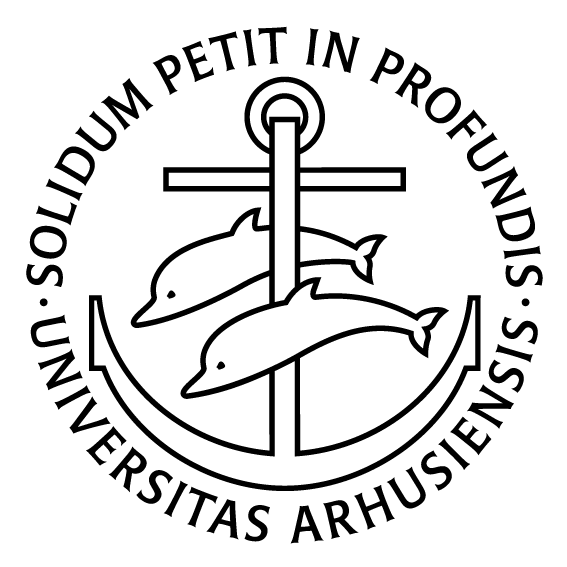
\includegraphics[width=0.45\textwidth]{latex/ausegl_sort}
        
        \vfill
        
    \end{center}
\end{titlingpage}

\newpage

\vspace*{\fill}

Copyright \textcopyright\,2019 \TeX nician and useR Andreas Kracht Frandsen

\textit{Typeset using Palatino Linotype}

\newpage

\pagenumbering{roman}

\tableofcontents

\newpage

\listoffigures

\newpage

\listoftables

\newpage

\hypertarget{preface}{%
\chapter*{Preface}\label{preface}}
\addcontentsline{toc}{chapter}{Preface}

This document answers Exercise 13, 16 and 22 of Handin 1 in the course Survival Analysis with SAS.

To see an interactive HTML version of this document, with the possibility to edit out mistakes or make comments, go to this website \href{https://afrandsen.rbind.io/bare/h1saws/index.html}{afrandsen.rbind.io/bare/h1saws.html}. It will be updated continuously if I find any mistakes myself through GitHub.

\newpage

\mainmatter

\pagenumbering{arabic}

\pagestyle{mypagestyle}

\setcounter{secnumdepth}{3}

\hypertarget{exercise-13}{%
\chapter{Exercise 13}\label{exercise-13}}

\emph{In this exercise we use the SAS data set houses again. Execute the following code.}

\begin{Shaded}
\begin{Highlighting}[]
\KeywordTok{PROC}\NormalTok{ GLM}\KeywordTok{ DATA}\NormalTok{ = houses;}
\NormalTok{CLASS new;}
\NormalTok{MODEL price = new size;}
\KeywordTok{OUTPUT}\NormalTok{ OUT = outdata PREDICTED = predvalues;}
\KeywordTok{RUN}\NormalTok{;}
\KeywordTok{QUIT}\NormalTok{;}
\end{Highlighting}
\end{Shaded}

\emph{Use the data set outdata to produce the same graphs as in Figure 5.1 and Figure 5.2 \citep{Pedersen2019}, noting in particular the ingenious choice of colors and symbols in the first figure. Save as pdf files.}

\hypertarget{sas-code}{%
\section{SAS Code}\label{sas-code}}

\hypertarget{the-houses-data-set}{%
\subsection{The Houses Data Set}\label{the-houses-data-set}}

In this exercise we use the data set \texttt{houses} which is obtained from the course website\footnote{Blackboard, Survival Analysis with SAS.}. Table \ref{tab:houses} shows the variables and the first 10 observations.

\begin{table}[!h]

\caption{\label{tab:houses}The first 10 observations of houses.txt.}
\centering
\begin{tabular}{lrrrrrr}
\toprule
  & taxes & beds & baths & new & price & size\\
\midrule
\rowcolor{gray!6}  1 & 3104 & 4 & 2 & 0 & 279.9 & 2048\\
2 & 1173 & 2 & 1 & 0 & 146.5 & 912\\
\rowcolor{gray!6}  3 & 3076 & 4 & 2 & 0 & 237.7 & 1654\\
4 & 1608 & 3 & 2 & 0 & 200.0 & 2068\\
\rowcolor{gray!6}  5 & 1454 & 3 & 3 & 0 & 159.9 & 1477\\
6 & 2997 & 3 & 2 & 1 & 499.9 & 3153\\
\rowcolor{gray!6}  7 & 4054 & 3 & 2 & 0 & 265.5 & 1355\\
8 & 3002 & 3 & 2 & 1 & 289.9 & 2075\\
\rowcolor{gray!6}  9 & 6627 & 5 & 4 & 0 & 587.0 & 3990\\
10 & 320 & 3 & 2 & 0 & 70.0 & 1160\\
\bottomrule
\end{tabular}
\end{table}

\hypertarget{import-of-the-houses-data-set}{%
\subsection{Import of the Houses Data Set}\label{import-of-the-houses-data-set}}

First we start by importing our data set to our SAS 9.4 session.

\begin{Shaded}
\begin{Highlighting}[]
\KeywordTok{DATA}\NormalTok{ houses;}
  \KeywordTok{INFILE} \StringTok{'~/Survival Analysis/Supplementary Notes/houses.txt'} 
\NormalTok{   FIRSTOBS = }\DecValTok{2}\NormalTok{;}
  \KeywordTok{INPUT}\NormalTok{ case taxes beds baths new price size;}
\KeywordTok{RUN}\NormalTok{;}
\end{Highlighting}
\end{Shaded}

Thus we take use of the \texttt{DATA} step. First we pass on the path to our data using the \texttt{INFILE} statement. Since our observations start in the second row, we must use the \texttt{FIRSTOBS} argument to tell SAS to start reading observations from the second row, by setting it to \texttt{2}. Next we tell SAS which columns and thereby variables in the \texttt{houses} data set it should read. We want every variable even though we aren't going to use all of them. Thus we use the \texttt{INPUT} statement which takes variables as arguments. \citep{DATAStep}

\hypertarget{model-fitting}{%
\subsection{Model Fitting}\label{model-fitting}}

Next we run the \texttt{GLM} procedure as stated in the exercise.

\begin{Shaded}
\begin{Highlighting}[]
\KeywordTok{PROC}\NormalTok{ GLM}\KeywordTok{ DATA}\NormalTok{ = houses;}
\NormalTok{CLASS new;}
\NormalTok{MODEL price = new size;}
\KeywordTok{OUTPUT}\NormalTok{ OUT = outdata PREDICTED = predvalues;}
\KeywordTok{RUN}\NormalTok{;}
\KeywordTok{QUIT}\NormalTok{;}
\end{Highlighting}
\end{Shaded}

We obtain the new data set \texttt{outdata} which is the same as the houses data set, but with an extra variable \texttt{predvalues} with the predicted prices. This variable can be spotted in Table \ref{tab:outdata} below.

\begin{table}[!h]

\caption{\label{tab:outdata}The first 10 observations of outdata.sas7bdat.}
\centering
\begin{tabular}{lrrrrrrr}
\toprule
  & taxes & beds & baths & new & price & size & predvalues\\
\midrule
\rowcolor{gray!6}  1 & 3104 & 4 & 2 & 0 & 279.9 & 2048 & 197.6\\
2 & 1173 & 2 & 1 & 0 & 146.5 & 912 & 65.7\\
\rowcolor{gray!6}  3 & 3076 & 4 & 2 & 0 & 237.7 & 1654 & 151.9\\
4 & 1608 & 3 & 2 & 0 & 200.0 & 2068 & 199.9\\
\rowcolor{gray!6}  5 & 1454 & 3 & 3 & 0 & 159.9 & 1477 & 131.3\\
6 & 2997 & 3 & 2 & 1 & 499.9 & 3153 & 383.7\\
\rowcolor{gray!6}  7 & 4054 & 3 & 2 & 0 & 265.5 & 1355 & 117.1\\
8 & 3002 & 3 & 2 & 1 & 289.9 & 2075 & 258.5\\
\rowcolor{gray!6}  9 & 6627 & 5 & 4 & 0 & 587.0 & 3990 & 423.1\\
10 & 320 & 3 & 2 & 0 & 70.0 & 1160 & 94.5\\
\bottomrule
\end{tabular}
\end{table}

\hypertarget{creation-of-plots}{%
\subsection{Creation of Plots}\label{creation-of-plots}}

\begin{Shaded}
\begin{Highlighting}[]
\NormalTok{ODS }\FunctionTok{PDF} \KeywordTok{FILE}\NormalTok{ = }\StringTok{'~/Survival Analysis/Supplementary Notes/Graph1.pdf'}\NormalTok{ NOTOC;}
\KeywordTok{OPTIONS}\NormalTok{ NODATE NONUMBER;}

\NormalTok{ODS GRAPHICS }\KeywordTok{ON}\NormalTok{ / NOBORDER}
\NormalTok{                  ATTRPRIORITY=NONE}
\NormalTok{                  WIDTH=9IN;}

\KeywordTok{PROC}\NormalTok{ SGPLOT}\KeywordTok{ DATA}\NormalTok{ = outdata;}
\NormalTok{SCATTER }\KeywordTok{X}\NormalTok{ = size Y = price / }\KeywordTok{GROUP}\NormalTok{ = new;}

\NormalTok{STYLEATTRS DATASYMBOLS=(TRIANGLE STAR)}
\NormalTok{           DATACONTRASTCOLORS=(BLUE ORANGE);}
           
\NormalTok{REG }\KeywordTok{X}\NormalTok{ = size Y = predvalues / }\KeywordTok{GROUP}\NormalTok{ = new}
\NormalTok{                              NOMARKERS}
\NormalTok{                              LINEATTRS=(PATTERN=SOLID);}
\NormalTok{YAXIS }\KeywordTok{LABEL}\NormalTok{ = }\StringTok{"Selling price"}\NormalTok{;}
\NormalTok{XAXIS }\KeywordTok{LABEL}\NormalTok{ = }\StringTok{"Size"}\NormalTok{;}
\NormalTok{KEYLEGEND / NOBORDER DOWN = }\DecValTok{2}\NormalTok{;}
\KeywordTok{RUN}\NormalTok{;}

\NormalTok{ODS GRAPHICS / }\KeywordTok{RESET}\NormalTok{ = ALL;}
\NormalTok{ODS GRAPHICS OFF;}

\NormalTok{ODS }\FunctionTok{PDF} \FunctionTok{CLOSE}\NormalTok{;}

\NormalTok{ODS }\FunctionTok{PDF} \KeywordTok{FILE}\NormalTok{ = }\StringTok{'~/Survival Analysis/Supplementary Notes/Graph2.pdf'}\NormalTok{ NOTOC;}
\KeywordTok{OPTIONS}\NormalTok{ NODATE NONUMBER;}

\NormalTok{ODS GRAPHICS }\KeywordTok{ON}\NormalTok{ / NOBORDER HEIGHT = 9IN;}

\KeywordTok{PROC}\NormalTok{ SGPANEL}\KeywordTok{ DATA}\NormalTok{ = outdata;}
\NormalTok{PANELBY new / COLUMNS = }\DecValTok{2}
\NormalTok{              ROWS = }\DecValTok{1}\NormalTok{;}
\NormalTok{SCATTER }\KeywordTok{X}\NormalTok{ = size Y = price;}
\NormalTok{REG }\KeywordTok{x}\NormalTok{ = size y = predvalues / NOMARKERS;}
\NormalTok{ROWAXIS }\KeywordTok{LABEL}\NormalTok{ = }\StringTok{"Selling price"}\NormalTok{;}
\NormalTok{COLAXIS }\KeywordTok{LABEL}\NormalTok{ = }\StringTok{"Size"}\NormalTok{;}
\NormalTok{KEYLEGEND / NOBORDER;}
\KeywordTok{RUN}\NormalTok{;}

\NormalTok{ODS GRAPHICS / }\KeywordTok{RESET}\NormalTok{ = ALL;}
\NormalTok{ODS GRAPHICS OFF;}

\NormalTok{ODS }\FunctionTok{PDF} \FunctionTok{CLOSE}\NormalTok{;}
\end{Highlighting}
\end{Shaded}

\hypertarget{plots}{%
\section{Plots}\label{plots}}

\hypertarget{the-first-figure}{%
\subsection{The First Figure}\label{the-first-figure}}

Figure \ref{fig:Graph-1} below show the pdf output achieved from the first \texttt{ODS\ PDF} statement in the SAS code from Section \ref{creation-of-plots}.\footnote{Yes, the caption is correctly positioned. I want to explicitly show the `A4' size from \texttt{ODS\ PDF}, and has thereby not scaled the pdf.}

Figure \ref{fig:Graph-1} below show the svg output achieved from the first \texttt{ODS\ GRAPHICS} statement in the SAS code from Appendix .\footnote{Notice the infinite scaling of svg output.}

\newpage

\begin{figure}[htbp!]

{\centering 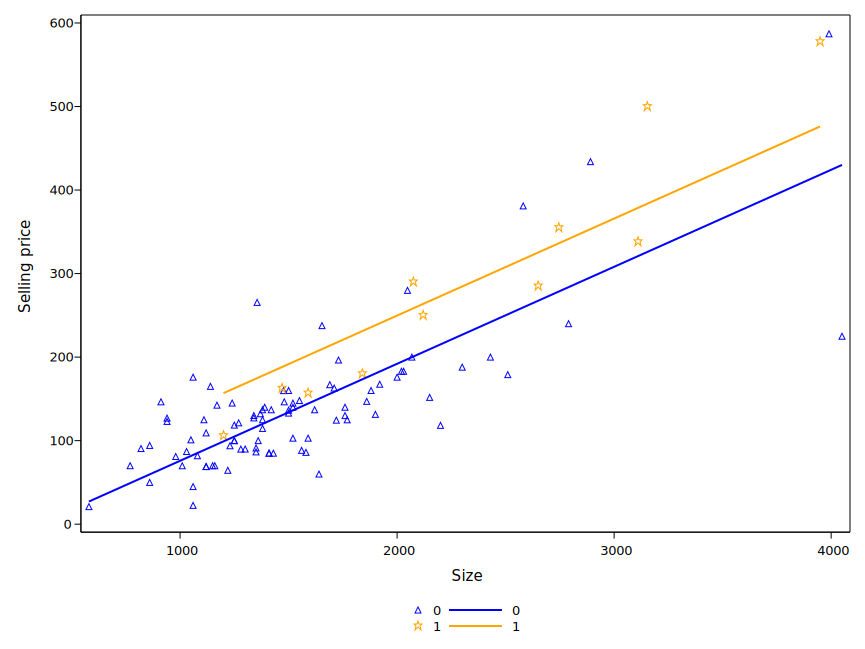
\includegraphics[width=1\linewidth]{graphs/EX13_G1} 

}

\caption{Output from the SGPlot Procedure.}\label{fig:Graph-1}
\end{figure}

\newpage

\hypertarget{the-second-figure}{%
\subsection{The Second Figure}\label{the-second-figure}}

Figure \ref{fig:Graph-2} below show the pdf output achieved from the second \texttt{ODS\ PDF} statement in the SAS code from Section \ref{creation-of-plots}.

Figure \ref{fig:Graph-2} below show the svg output achieved from the second \texttt{ODS\ GRAPHICS} statement in the SAS code from Appendix .

\newpage

\begin{figure}[htbp!]

{\centering 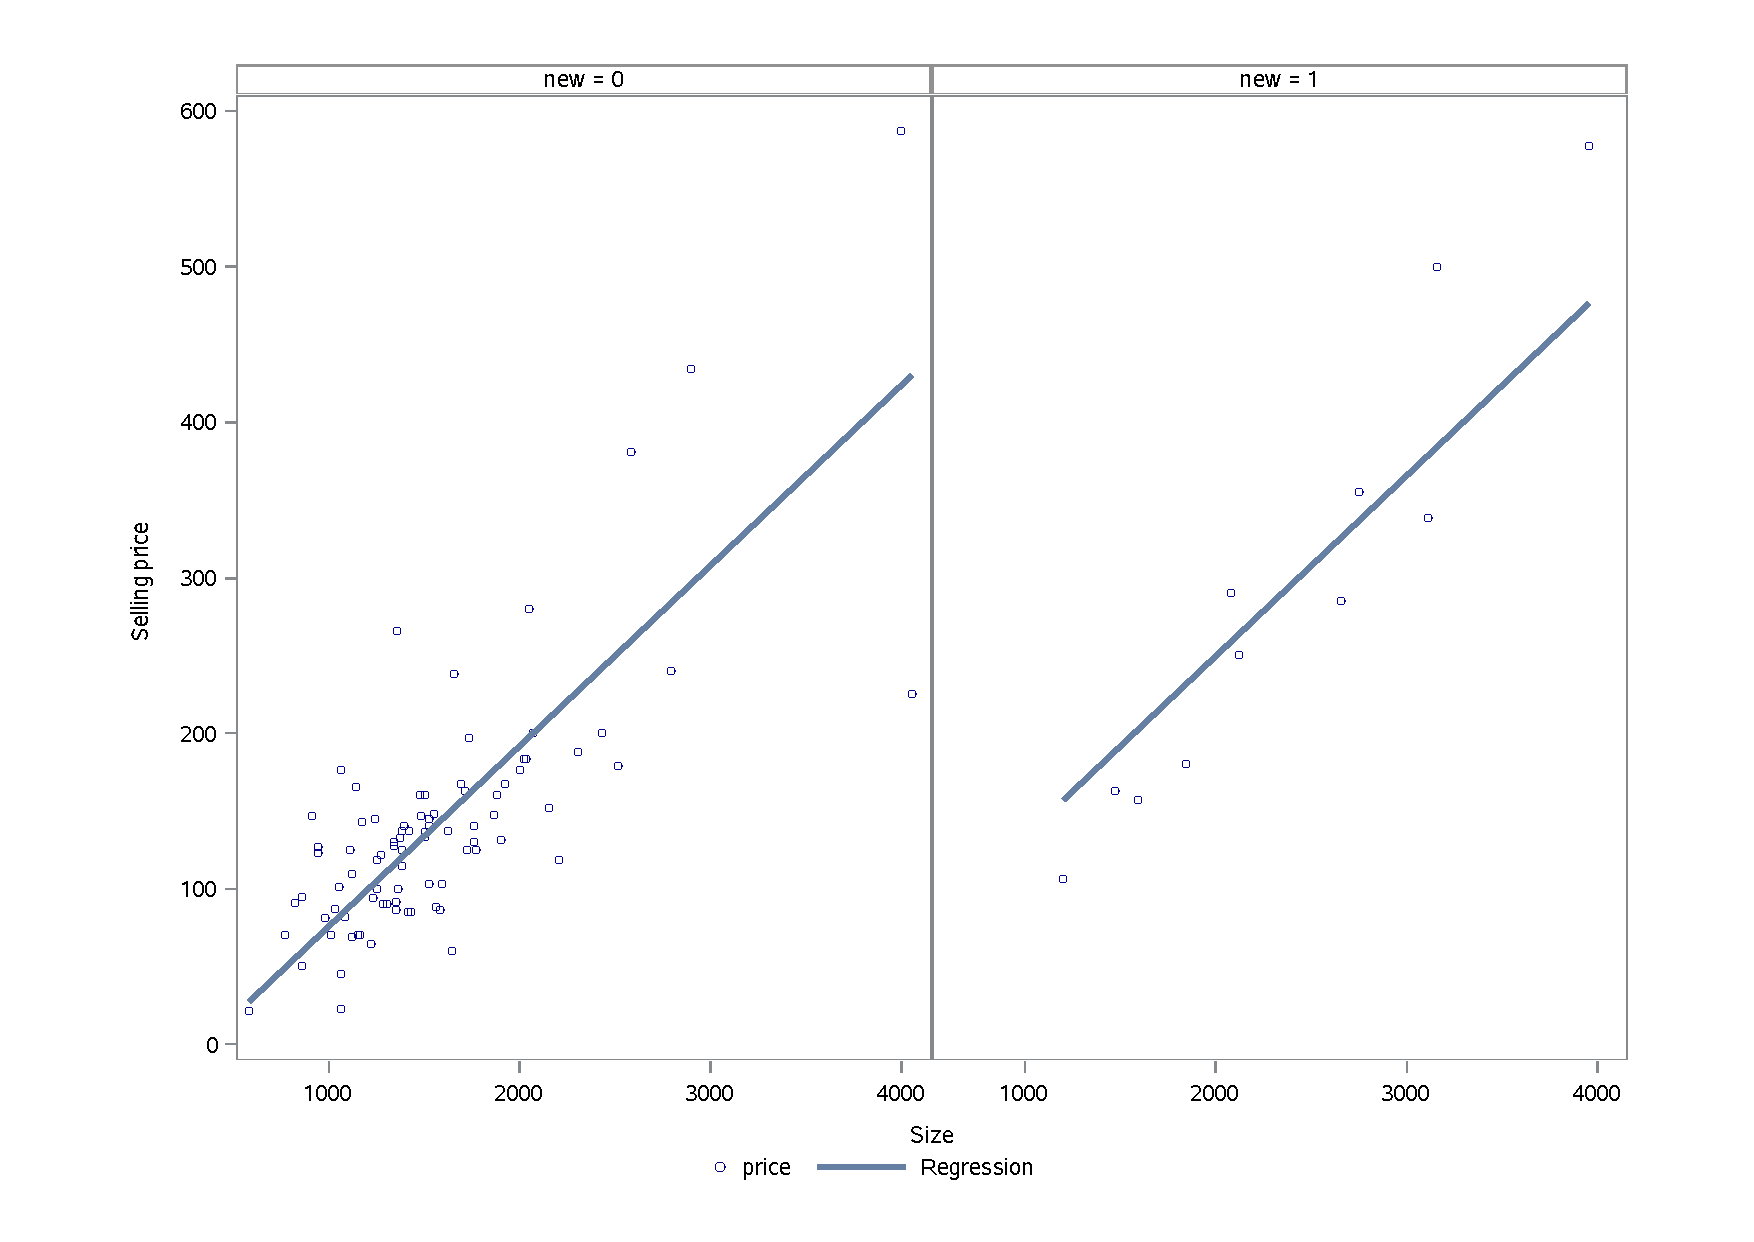
\includegraphics[width=1\linewidth]{graphs/EX13_G2} 

}

\caption{Output from the SGPanel Procedure.}\label{fig:Graph-2}
\end{figure}

\newpage

We notice that Figure \ref{fig:Graph-1} and Figure \ref{fig:Graph-2} are indeed equal to Figure 5.1 and Figure 5.2 \citep{Pedersen2019}.

\newpage

\hypertarget{exercise-16}{%
\chapter{Exercise 16}\label{exercise-16}}

\emph{Exercise 1.21 \citep{Agresti2015} presented a study comparing forced expiratory volume after 1 hour of treatment for three drugs (\(a\), \(b\), and \(p = \text{placebo}\)), adjusting for a baseline measurement \(x_1\). Table 4.1 \citep{Agresti2015} shows the results of fitting some normal GLMs (with identity link, except one with log link) and a GLM assuming a gamma response. Interpret results.}

\begin{enumerate}
\def\labelenumi{\arabic{enumi}.}
\item
  \emph{Do all analyses in SAS}
\item
  \emph{Write up the models mathematically.}
\item
  \emph{Include graphs to illustrate (lack of) fit.}
\item
  \emph{Which models (or which model) seem to perform best?}
\end{enumerate}

The dataset \texttt{FEV} is obtained from \citep{FEV}. Table \ref{tab:FEV} shows the variables and the first 10 observations.

\begin{table}[!h]

\caption{\label{tab:FEV}The first 10 observations of FEV.dat.}
\centering
\begin{tabular}{lrrrrrrrrrr}
\toprule
  & base & fev1 & fev2 & fev3 & fev4 & fev5 & fev6 & fev7 & fev8 & drug\\
\midrule
\rowcolor{gray!6}  1 & 2.46 & 2.68 & 2.76 & 2.50 & 2.30 & 2.14 & 2.40 & 2.33 & 2.20 & a\\
2 & 3.50 & 3.95 & 3.65 & 2.93 & 2.53 & 3.04 & 3.37 & 3.14 & 2.62 & a\\
\rowcolor{gray!6}  3 & 1.96 & 2.28 & 2.34 & 2.29 & 2.43 & 2.06 & 2.18 & 2.28 & 2.29 & a\\
4 & 3.44 & 4.08 & 3.87 & 3.79 & 3.30 & 3.80 & 3.24 & 2.98 & 2.91 & a\\
\rowcolor{gray!6}  5 & 2.80 & 4.09 & 3.90 & 3.54 & 3.35 & 3.15 & 3.23 & 3.46 & 3.27 & a\\
6 & 2.36 & 3.79 & 3.97 & 3.78 & 3.69 & 3.31 & 2.83 & 2.72 & 3.00 & a\\
\rowcolor{gray!6}  7 & 1.77 & 3.82 & 3.44 & 3.46 & 3.02 & 2.98 & 3.10 & 2.79 & 2.88 & a\\
8 & 2.64 & 3.67 & 3.47 & 3.19 & 2.19 & 2.85 & 2.68 & 2.60 & 2.73 & a\\
\rowcolor{gray!6}  9 & 2.30 & 4.12 & 3.71 & 3.57 & 3.49 & 3.64 & 3.38 & 2.28 & 3.72 & a\\
10 & 2.27 & 2.77 & 2.77 & 2.75 & 2.75 & 2.71 & 2.75 & 2.52 & 2.60 & a\\
\bottomrule
\end{tabular}
\end{table}

\hypertarget{models}{%
\section{Models}\label{models}}

We will study the following models

\hypertarget{additive-model-base}{%
\subsection{Additive Model -- base}\label{additive-model-base}}

\[Y_{ij}\sim N\left(\alpha + \gamma b_{ij}, \sigma^2\right),\]

where \(i=a,b,p\), \(j=1,\dots,24\).

The above model is a NLM with \(\beta=\left(\alpha, \gamma \right)^\textsf{T}\).

\hypertarget{additive-model-drug}{%
\subsection{Additive Model -- drug}\label{additive-model-drug}}

\[Y_{ij}\sim N\left(\alpha + \beta_{i}, \sigma^2\right),\]

where \(i=a,b,p\), \(j=1,\dots,24\).

The above model is a NLM with \(\beta=\left(\alpha, \beta_{a}, \beta_b, \beta_p \right)^\textsf{T}\).

\hypertarget{additive-model-basedrug}{%
\subsection{Additive Model -- base+drug}\label{additive-model-basedrug}}

\[Y_{ij}\sim N\left(\alpha + \gamma b_{ij} + \beta_{i}, \sigma^2\right),\]

where \(i=a,b,p\), \(j=1,\dots,24\).

The above model is a NLM with \(\beta=\left(\alpha, \gamma, \beta_{a}, \beta_b, \beta_p \right)^\textsf{T}\).

\hypertarget{additive-model-basedrug-gamma}{%
\subsection{Additive Model -- base+drug (gamma)}\label{additive-model-basedrug-gamma}}

\[Y_{ij}\sim \Gamma\left(\alpha + \gamma b_{ij} + \beta_{i}, k\right),\]

where \(i=a,b,p\), \(j=1,\dots,24\).

\hypertarget{additive-model-basedrug-log-link}{%
\subsection{Additive Model -- base+drug (log link)}\label{additive-model-basedrug-log-link}}

\[Y_{ij}\sim N\left(\mu_{ij}, \sigma^2\right),\]

where \(i=a,b,p\), \(j=1,\dots,24\).

\[\mu_{ij}=\log(\mathbb{E}(Y_{ij}))=\alpha + \gamma b_{ij} + \beta_{i}.\]

The above model is a NLM with \(\beta=\left(\alpha, \gamma, \beta_{a}, \beta_b, \beta_p \right)^\textsf{T}\).

\hypertarget{interaction-model-basedrugbasedrug}{%
\subsection{Interaction Model -- base+drug+base*drug}\label{interaction-model-basedrugbasedrug}}

\[Y_{ij}\sim N\left(\alpha + \gamma b_{ij} + \beta_{i} + \delta_i b_{ij}, \sigma^2\right),\]

where \(i=a,b,p\), \(j=1,\dots,24\).

The above model is a NLM with \(\beta=\left(\alpha, \gamma, \beta_{a}, \beta_b, \beta_p, \delta_a, \delta_b, \delta_p \right)^\textsf{T}\).

\newpage

\hypertarget{exercise-22}{%
\chapter{Exercise 22}\label{exercise-22}}

\emph{Let \(X\) have a Weibull distribution with parameters \(\alpha, \lambda > 0\), that is, \(X\) has density \(f\) as indicated in Table 2.2 in \citet{Klein2003}.}

\hypertarget{question-1}{%
\section{Question 1}\label{question-1}}

\emph{Show that \(h\) and \(S\) are as indicated in \citet{Klein2003}, Table 2.2. Determine \(H\) as well.}

\hypertarget{weibull-distributed-random-variable}{%
\subsection{Weibull Distributed Random Variable}\label{weibull-distributed-random-variable}}

The random variable \(X \sim \text{Weibull}(\alpha, \lambda)\) with \(\alpha, \lambda > 0\), has the following probability density function

\begin{equation}
f(x) = \alpha\lambda x^{\alpha-1}\exp(-\lambda x^\alpha)\quad x\geq 0. \label{eq:PDF}
\end{equation}

\hypertarget{survival-function}{%
\subsection{Survival Function}\label{survival-function}}

For a continuous random variable the survival function is defined as the complement of the cumulative distribution function

\begin{equation}
S(x)=1-F(x)=P(X>x)=\int^{\infty}_x f(t) dt. \label{eq:Surv}
\end{equation}

Thus for the continouos random variable \(X\) we use Equation \eqref{eq:Surv}.

We insert Equation \eqref{eq:PDF} in Equation \eqref{eq:Surv} and perform the calculation for \(x\geq 0\).

\begin{align}
S(x)&=\int^{\infty}_x \alpha\lambda t^{\alpha-1}\exp(-\lambda t^\alpha) dt \notag \\
    &=\alpha\lambda\int^{\infty}_x t^{\alpha-1}\exp(-\lambda t^\alpha) dt \notag \\
    &=\alpha\lambda\int_{x^{\alpha}}^\infty t^{\alpha-1}\exp(-\lambda u) \frac{1}{\alpha t^{\alpha-1}} du \notag \\
    &=\lambda \int_{x^{\alpha}}^\infty \exp(-\lambda u) du \notag \\
    &=\left[-\exp\left(-\lambda u\right)\right]_{x^\alpha}^\infty \notag \\
    &=\left(-\exp(-\lambda\cdot \infty)-(-\exp(-\lambda\cdot x^\alpha))\right) \notag \\
    &=\left(0-(-\exp(-\lambda\cdot x^\alpha))\right) \notag \\
    &=\exp(-\lambda x^\alpha) \label{eq:WeiSurv}.
\end{align}

Where we in the third and fifth equality perform integration by substitution. We see that the above function is indeed equal to the survival function in Table 2.2 \citep{Klein2003}.

\hypertarget{hazard-function}{%
\subsection{Hazard Function}\label{hazard-function}}

For a continuous random variable the hazard function (rate) is defined as

\begin{equation}
h(x)= \frac{f(x)}{S(x)}. \label{eq:Hazard}
\end{equation}

We insert Equation \eqref{eq:WeiSurv} and Equation \eqref{eq:PDF} in Equation \eqref{eq:Hazard} and perform the calculation for \(x\geq 0\).

\begin{align}
h(x)&= \frac{f(x)}{S(x)} \notag \\
    &=\frac{\alpha\lambda x^{\alpha-1}\exp(-\lambda x^\alpha)}{\exp(-\lambda x^\alpha)} \notag \\
    &=\alpha\lambda x^{\alpha-1}. \label{eq:WeiHazard}
\end{align}

We see that the above function is indeed equal to the hazard function in Table 2.2 \citep{Klein2003}.

\hypertarget{cumulative-hazard-function}{%
\subsection{Cumulative Hazard Function}\label{cumulative-hazard-function}}

For a continuous random variable the cumulative hazard function is defined as

\begin{equation}
H(x)= \int_0^x h(u) du = -\ln(S(x)). \label{eq:CumuHazard}
\end{equation}

We insert Equation \eqref{eq:WeiSurv} in Equation \eqref{eq:CumuHazard} and perform the calculation for \(x\geq 0\).

\begin{equation}
H(x) = -\ln(\exp(-\lambda x^\alpha))=\lambda x^\alpha. \label{eq:WeiCumuHazard}
\end{equation}

We see that the above function is indeed equal to the cumulative hazard function in (\citet{Klein2003}, page 32).

Thus we showed that the functions in Table 2.2 \citep{Klein2003} are correct and we are done.

\hypertarget{question-2}{%
\section{Question 2}\label{question-2}}

\emph{Determine the distribution of \(X^\gamma\) for \(\gamma > 0\).}

We calculate the survival function of \(X^\gamma\). Since the distribution of a random variable is fully described by it's survival function.

\begin{align}
S_{X^{\gamma}}(x)&=P\left(X^\gamma>x\right) \notag\\
                 &=P\left(\ln(X^\gamma)>\ln(x)\right) \notag\\
                 &=P\left(\gamma\ln(X)>\ln(x)\right) \notag\\
                 &=P\left(\ln(X)>\frac{\ln(x)}{\gamma}\right) \notag\\
                 &=P\left(\exp(\ln(X))>\exp\left(\frac{\ln(x)}{\gamma}\right)\right) \notag\\
                 &=P\left(X>\exp\left(\frac{\ln(x)}{\gamma}\right)\right) \notag\\
                 &=S_X\left(\exp\left(\frac{\ln(x)}{\gamma}\right)\right) \notag\\
                 &=\exp\left(-\lambda \left(\exp\left(\frac{\ln(x)}{\gamma}\right)\right)^\alpha\right) \notag\\
                 &=\exp\left(-\lambda x^{\tfrac{\alpha}{\gamma}}\right). \label{eq:WeiGammaSurv}
\end{align}

Thus from Table 2.2 \citep{Klein2003} we have \(X^\gamma\sim \text{Weibull}\left(\frac{\alpha}{\gamma},\lambda\right)\).

\hypertarget{question-3}{%
\section{Question 3}\label{question-3}}

\emph{Determine the distribution of \(\lambda X^\alpha\).}

We calculate the survival function of \(\lambda X^\alpha\). Since the distribution of a random variable is fully described by it's survival function.

\begin{align}
S_{\lambda X^{\alpha}}(x)&=P\left(\lambda X^{\alpha}>x\right) \notag\\
                 &=P\left(\ln(\lambda X^{\alpha})>\ln(x)\right) \notag\\
                 &=P\left(\ln(\lambda)+\alpha\ln(X)>\ln(x)\right) \notag\\
                 &=P\left(\ln(X)>\frac{\ln(x)-\ln(\lambda)}{\alpha}\right) \notag\\
                 &=P\left(\exp(\ln(X))>\exp\left(\frac{\ln(x)-\ln(\lambda)}{\alpha}\right)\right) \notag\\
                 &=P\left(X>\exp\left(\frac{\ln(x)-\ln(\lambda)}{\alpha}\right)\right) \notag\\
                 &=S_X\left(\exp\left(\frac{\ln(x)-\ln(\lambda)}{\alpha}\right)\right) \notag\\
                 &=\exp\left(-\lambda\left(\exp\left(\frac{\ln(x)-\ln(\lambda)}{\alpha}\right)\right)^\alpha\right) \notag\\
                 &=\exp\left(-\lambda x^{\tfrac{\alpha}{\gamma}}\right) \notag\\
                 &=\exp(-x). \label{eq:WeiOneSurv}
\end{align}

Thus from Table 2.2 \citep{Klein2003} we have \(\lambda X^\alpha\sim \text{Weibull}\left(1,1\right) \overset{\text{d}}{=} \text{Exp}(1)\).

Figure \ref{fig:WeiDist} below show the distribution.

\begin{figure}[htbp!]

{\centering 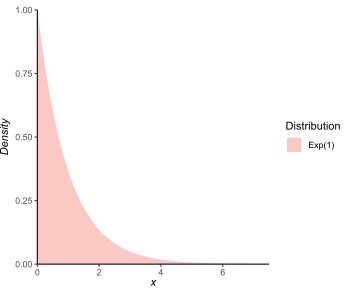
\includegraphics{Handin_1_Andreas_Kracht_Frandsen_files/figure-latex/WeiDist-1} 

}

\caption{Density of a Exp(1) distribution.}\label{fig:WeiDist}
\end{figure}

\hypertarget{question-4}{%
\section{Question 4}\label{question-4}}

\emph{Let \(n\in\mathbb{N}\) and \(X_1,\dots,X_n\) be i.i.d. and have a Weibull distribution with parameters \(\alpha, \lambda > 0\) as common distribution. Determine the distribution of \(\min(X_1,\dots,X_n)\).}

The random variable \(X_i\) has the survival function

\[S_{X_i}(x)=\exp(-\lambda x^\alpha)\quad x\geq 0,\]

for \(i=1,2,\dots,n\). As proved in Section \ref{survival-function}, Equation \eqref{eq:WeiSurv}.

Let \(Y=\min(X_1,\dots,X_n)\), then the survival function of \(Y\) is

\begin{align}
S_Y(y)&=P(Y>y) \notag\\
      &=P(\min(X_1,\dots,X_n)>y) \notag\\
      &=P(X_1>y,X_2>y,\dots,X_n>y) \notag\\
      &=P(X_1>y)\cdot P(X_1>y)\cdots P(X_n>y) \notag\\
      &=S_{X_1}(y)\cdot S_{X_2}(y)\cdots S_{X_n}(y) \notag\\
      &=(\exp(-\lambda y^\alpha))\cdot (\exp(-\lambda y^\alpha))\cdots \exp(-\lambda y^\alpha) \notag\\
      &=\exp(-n\cdot\lambda y^\alpha). \label{eq:WeiMinSurv}
\end{align}

Where we in the fourth equality take use of the independency of our random variables. Thus \(Y=\min(X_1,\dots,X_n)\sim \text{Weibull}(\alpha, n\lambda)\).

\newpage

\hypertarget{appendix-appendix}{%
\appendix}


\hypertarget{sas-code-of-exercise-16}{%
\chapter{SAS Code of Exercise 16}\label{sas-code-of-exercise-16}}

\hypertarget{code-a}{%
\section{Code A}\label{code-a}}

\hypertarget{code-aa}{%
\subsection{Code AA}\label{code-aa}}

\begin{Shaded}
\begin{Highlighting}[]
\KeywordTok{data}\NormalTok{ fev;}
  \KeywordTok{infile} \StringTok{'~/Survival Analysis/Supplementary Notes/FEV.dat'} 
\NormalTok{   firstobs=}\DecValTok{2}\NormalTok{;}
  \KeywordTok{input}\NormalTok{ patient base fev1 fev2 fev3 fev4 fev5 fev6 fev7 fev8 drug $}\DecValTok{1}\NormalTok{.;}
\KeywordTok{RUN}\NormalTok{;}

\CommentTok{* AIC = 134.4;}
\KeywordTok{proc}\NormalTok{ genmod}\KeywordTok{ data}\NormalTok{=fev plots=all;}
\NormalTok{class drug;}
\NormalTok{model fev1 = base / dist=}\FunctionTok{normal} \KeywordTok{link}\NormalTok{=identity;}
\KeywordTok{run}\NormalTok{;}

\CommentTok{* AIC = 152.4;}
\KeywordTok{proc}\NormalTok{ genmod}\KeywordTok{ data}\NormalTok{=fev plots=all;}
\NormalTok{class drug(ref=}\StringTok{'a'}\NormalTok{);}
\NormalTok{model fev1 = drug / dist=}\FunctionTok{normal} \KeywordTok{link}\NormalTok{=identity;}
\KeywordTok{run}\NormalTok{;}

\CommentTok{* AIC = 103.4;}
\KeywordTok{proc}\NormalTok{ genmod}\KeywordTok{ data}\NormalTok{=fev plots=all;}
\NormalTok{class drug(ref=}\StringTok{'a'}\NormalTok{);}
\NormalTok{model fev1 = base drug / dist=}\FunctionTok{normal} \KeywordTok{link}\NormalTok{=identity;}
\KeywordTok{run}\NormalTok{;}

\CommentTok{* AIC = 106.2;}
\KeywordTok{proc}\NormalTok{ genmod}\KeywordTok{ data}\NormalTok{=fev plots=all;}
\NormalTok{class drug(ref=}\StringTok{'a'}\NormalTok{);}
\NormalTok{model fev1 = base drug / dist=}\FunctionTok{gamma} \KeywordTok{link}\NormalTok{=identity;}
\KeywordTok{run}\NormalTok{;}

\CommentTok{* AIC = 106.8;}
\KeywordTok{proc}\NormalTok{ genmod}\KeywordTok{ data}\NormalTok{=fev plots=all;}
\NormalTok{class drug(ref=}\StringTok{'a'}\NormalTok{);}
\NormalTok{model fev1 = base drug / dist=}\FunctionTok{normal} \KeywordTok{link}\NormalTok{=}\FunctionTok{log}\NormalTok{;}
\KeywordTok{run}\NormalTok{;}

\CommentTok{* AIC = 107.1;}
\KeywordTok{proc}\NormalTok{ genmod}\KeywordTok{ data}\NormalTok{=fev plots=all;}
\NormalTok{class drug(ref=}\StringTok{'a'}\NormalTok{);}
\NormalTok{model fev1 = base drug base*drug / dist=}\FunctionTok{normal} \KeywordTok{link}\NormalTok{=identity;}
\KeywordTok{run}\NormalTok{;}
\end{Highlighting}
\end{Shaded}

\newpage

\nocite{*}

\bibliography{references.bib}


\end{document}
